% !TEX root = ../neurosciences-barrels.tex

\section{Material and methods}

%%%%%%%%%%%%%%%%%%%%%%%%%%%%%%%%%%%%%%%%%%%%%%%%%%%
%%%%%%%%%%%%%%%%%%%%%%%%%%%%%%%%%%%%%%%%%%%%%%%%%%%
%%%%%%%%%%%%%%%%%%%%%%%%%%%%%%%%%%%%%%%%%%%%%%%%%%%
\subsection{Overview of the proposed framework}
\label{sec-overview}

This Section details each step of the proposed method. The corresponding Matlab code to reproduce the figures of this article is available online\footnote{\url{https://github.com/gpeyre/2014-NeuroMeth-barrels}}. This code is packaged as a graphical user interface (GUI) that is helpful to guide the user through the various processing steps, from image loading to the final reconstructed barrel map. 

Table~\ref{table-notations} reviews the notation introduced in the paper. Table~\ref{table-parameters} lists the parameters of the method, together with the default values used in our numerical simulations. � 

\newcommand{\notation}[3]{ $#1$ & #2 & #3 \\ }


%%%%%%%%%%%%%%%%%%%%%%%%%%%%%%%%%%%%%%%%%%%%%%%%
\begin{listing}[ht!]
%
\centering
\begin{tabular}{|c|c|c|}
	\hline
	Notation & & See  \\\hline
	\notation{ m \in \{1,\ldots,Q\} }{ Index of a slice }{ Sec~\ref{sec-registration} }
	\notation{\{S_1,\ldots,S_{Q}\} }{�Input slices }{�Sec~\ref{sec-registration} }
	\notation{\NCC}{�Norm. cross correlation }{�\ref{app-crosscorrel} }
	\notation{\Xx_m}{�Set of detected vessels }{�Sec~\ref{sec-vessel-detec} }
	\notation{\Relevant}{�Slices containing barrels }{�Sec~\ref{sec-grad-fusion} }
	\notation{\Tt_m}{�Registration map }{�Eq~\eqref{eq-def-registered-data} }  
	\notation{\{\tilde S_1,\ldots,\tilde S_{Q}\}}{Registered slices}{ Eq~\eqref{eq-def-registered-data} }
	\notation{\{\bar S_1,\ldots,\bar S_{Q}\}}{Inpainted slices}{Sec~\ref{sec-inpaint-denoise}}
	\notation{S}{Fused image}{Sec~\ref{sec-grad-fusion}}
	\notation{\bar S}{Drift-corrected result}{Eq~\eqref{eq-drift-removal}}
	\hline
\end{tabular}
% \notation{\Om}{Segmented barrel map}{Sec~\ref{sec-barrel-segmentation}}
%
\caption{ \label{table-notations} Notations used in the paper. } 
\end{listing}
%%%%%%%%%%%%%%%%%%%%%%%%%%%%%%%%%%%%%%%%%%%%%%%%

%%%%%%%%%%%%%%%%%%%%%%%%%%%%%%%%%%%%%%%%%%%%%%%%
\begin{listing}[ht!]
%
\centering
\begin{tabular}{|c|c|c|c|}
	\hline
	Param. & & See  & Default \\\hline
	$\tau$ & NCC threshold & Sec~\ref{sec-vessel-detec} & 0.75 \\
	$N$ & Max. number of vessels & Sec~\ref{sec-vessel-detec} & 30 \\
	$\si_{\max}$ & Maximum vessel radius & Sec~\ref{sec-vessel-detec} & 4.5 \\
	$\epsilon$ & ICP robustness parameter & Eq~\eqref{eq-weighting-robust} & -- \\
	$\si^\star$ & Width of debiasing kernel & Eq~\eqref{eq-drift-removal} & 10 \\\hline
\end{tabular}
%	$\la$ & Regul. of the segmentation & Sec~\ref{sec-barrel-segmentation} & ? \\
%
\caption{ Parameters used in the paper.}
\label{table-parameters}  
\end{listing}
%%%%%%%%%%%%%%%%%%%%%%%%%%%%%%%%%%%%%%%%%%%%%%%%

The successive steps of the algorithms are:
\begin{rs}
	\item Segment the foreground to obtain the input section images $\{S_1,\ldots,S_{Q}\}$
		(Section~\ref{sec-preprocessing}).
	\item For each $m \in \{1,\ldots,Q\}$, compute the list of detected vessel positions $\Xx_m$ 
		(Section~\ref{sec-vessel-detec}).
	\item For each $m \in \{1,\ldots,Q-1\}$, compute the optimal transform $T_m$ to register $S_m$ with $S_{m+1}$
		(Section~\ref{sec-icp-alignement}).
	\item Apply the transforms to obtain the registered images $\{\tilde S_1,\ldots,\tilde S_Q\}$
		(Equation~\eqref{eq-def-registered-data}).
	\item For each $m$, inpaint the detected vessel and denoise the resulting images to obtain $\{\bar S_1,\ldots,\bar S_Q\}$
		(Section~\ref{sec-inpaint-denoise}).
	\item Fuse the relevant maps  $\{\bar S_m\}_{m \in \Relevant}$ (where $\Mm \subset�\{1,\ldots,Q\}$ indexes the maps containing apparent barrels) to obtain the fused map $S$
		(Section~\ref{sec-grad-fusion}).		
	\item Remove the low frequency drift to obtain $\bar S$
		(Section~\ref{sec-drift-removal}). 
% 	\item Segment the map $\bar S$ to obtain the location $\Om$ of the barrels. 
\end{rs}


%%%%%%%%%%%%%%%%%%%%%%%%%%%%%%%%%%%%%%%%%%%%
%%%%%%%%%%%%%%%%%%%%%%%%%%%%%%%%%%%%%%%%%%%%
%%%%%%%%%%%%%%%%%%%%%%%%%%%%%%%%%%%%%%%%%%%%
\subsection{Step 1: Pairwise Registration of Histological Sections}
\label{sec-registration}


The input of the algorithm is $Q$ raw images which are digital images with range normalized in $[0,1]$ (0 being black and $1$ white). Figure~\ref{somatotopy}D shows examples of such images. 


%%%%%%%%%%%%%%%%%%%%%%%%%%%%%%%%%%%%%%%%%%%%
\subsubsection{Pre-processing}
\label{sec-preprocessing}

Depending on the configuration of the microscope used to acquire the images, the input images contain 2 or 3 regions:
\begin{rs}
	\item In the center of the image, a gray region corresponding to the histological section of the cortex. This is the foreground region.
	\item A circular white region corresponding to the lens/plate of the microscope and that surrounds the cortex region. It is considered as background.
	\item In some cases, a black region can also surround the two other regions. It is also considered as background.
\end{rs}
We extract the background using a $K$-means algorithm with $K=3$ regions.
%  This is a particular case of the region-based segmentation algorithm detailed in~\ref{app-segmentation}, where no regularization is used ($\la=0$). 
The background is then replaced by the value $0$ and the resulting images (the so-called ``slices'' in the following) are denoted $\{S_1,\ldots,S_Q \}$. 


%%%%%%%%%%%%%%%%%%%%%%%%%%%%%%%%%%%%%%%%%%%%
\subsubsection{Vessel Detection}
\label{sec-vessel-detec}

Blood vessels which are approximately orthogonal to the cutting plane look like slightly elliptic spots that can be approximated by small Gaussians. To be invariant to local contrast fluctuations, we detect these orthogonal vessels using normalized cross correlations with Gaussian templates of varying standard deviations, assumed to be smaller than $\si_{\max}$.

For each slice $S_m$, for $m \in \{1,\ldots,Q\}$, we compute its associated normalized cross correlation $\NCC(S_m)$ against the set of Gaussian templates, as detailed in~\ref{app-crosscorrel}. Given a threshold $\tau \in [0,1]$ and a maximum number $N$ of detected vessels, we define the detected vessel centers $\Xx_m$ to be the set of pixels $x$ satisfying both $\NCC(S_m)(x)>\tau$ and $\NCC(S_m)(x)$ is among the $N$ largest values of $\NCC(S_m)$. 


%%%%%%%%%%%%%%%%%%%%%%%%%%%%%%%%%%%%%%%%%%%%%%%%%%%
%%%%%%%%%%%%%%%%%%%%%%%%%%%%%%%%%%%%%%%%%%%%%%%%%%%
%%%%%%%%%%%%%%%%%%%%%%%%%%%%%%%%%%%%%%%%%%%%%%%%%%%
\subsubsection{Slice Registration by Robust ICP}
\label{sec-icp-alignement}

For each $m$, we now register the slice $S_m$ with the slice $S_{m+1}$ (see Figure~\ref{fig-algo-sample}A). Registration is obtained by computing an optimal transformation $T_m$ which maps pixels in slice $S_{m+1}$ to pixels in image $S_{m}$. We restrict here the computation to rigid transformations, i.e. of the form $T(x) = R(x) + t$ where $R$ is a planar rotation and $t \in \RR^2$ is a translation vector. 

\begin{figure}[ht!]
\centering
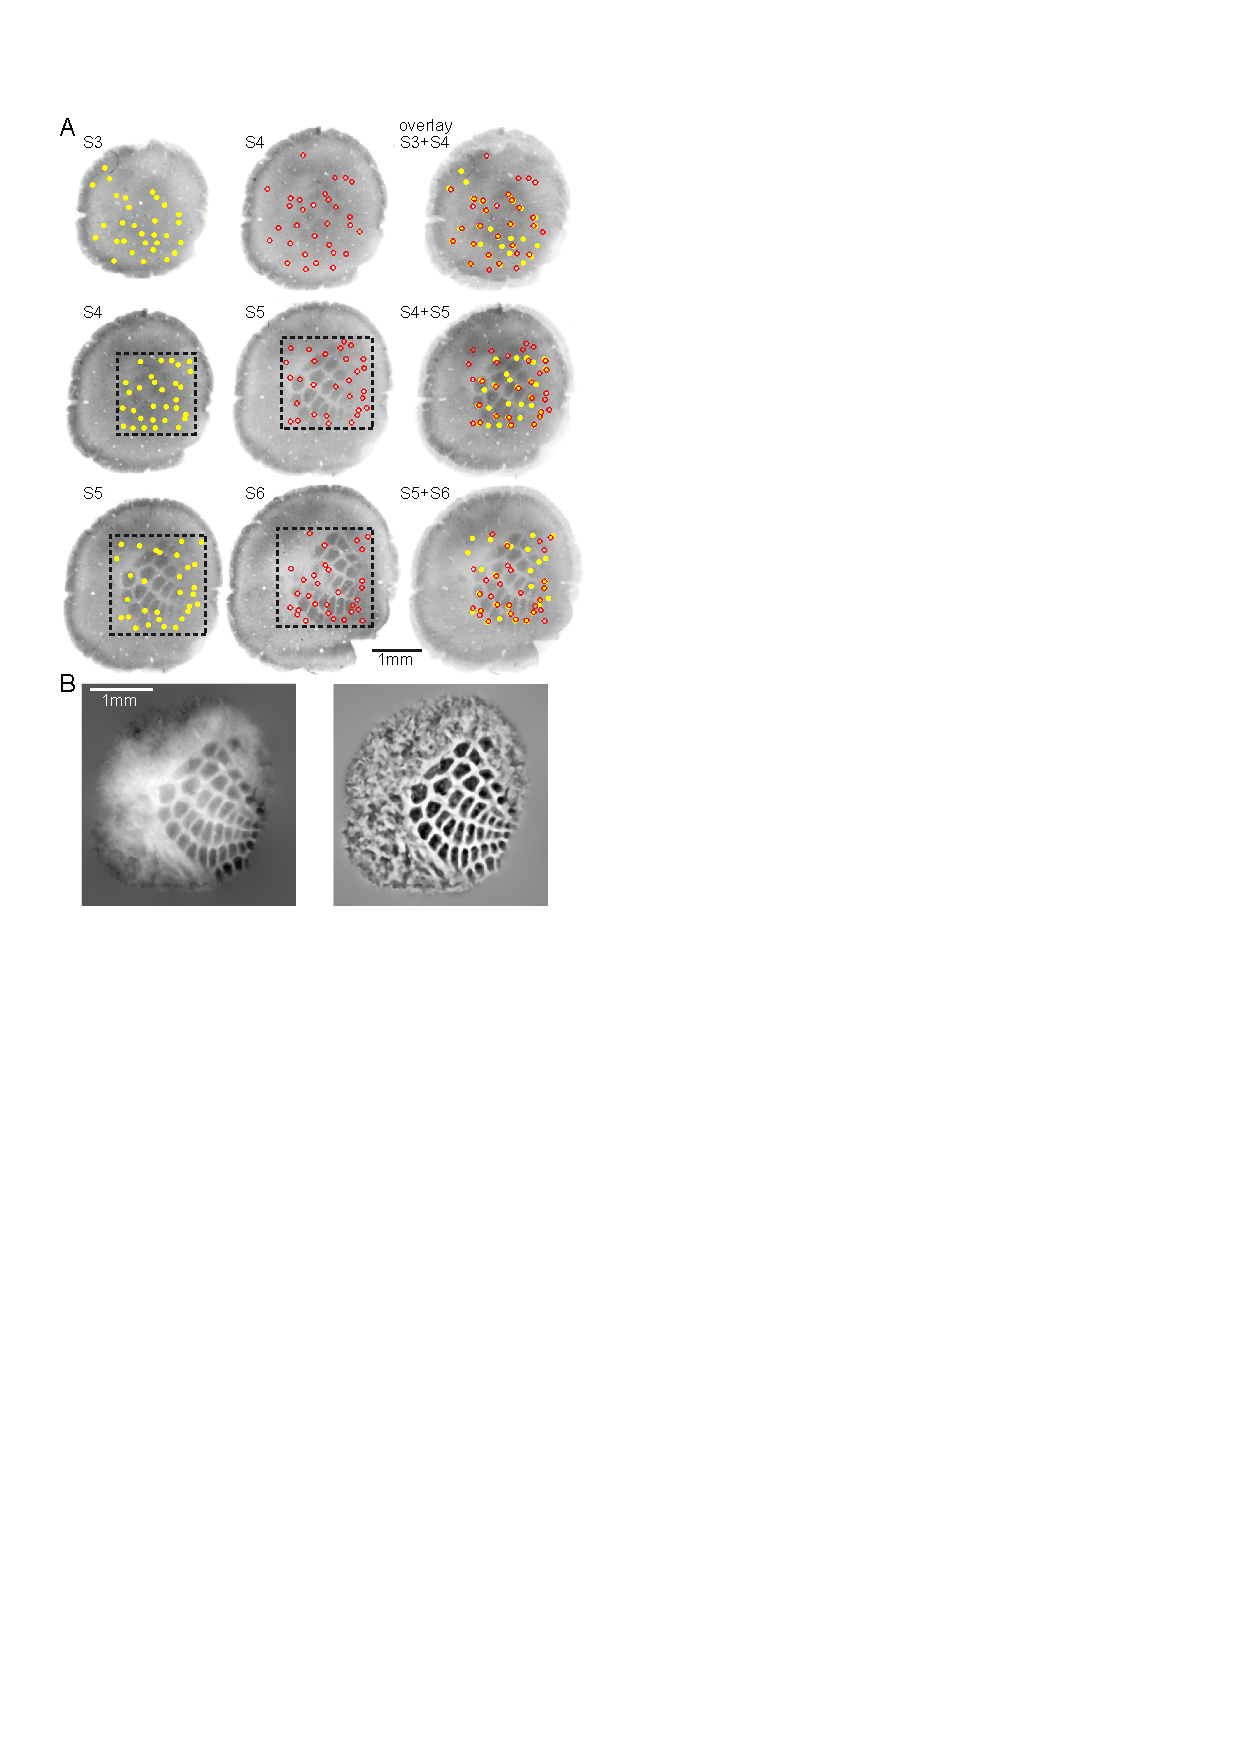
\includegraphics[width=89mm]{images/Perronnet-Figure3}
\caption{
	\textbf{Registration of histological slices and subsequent barrel map reconstruction. }\\
	%
	\textbf{A.} Snapshots extracted from the GUI illustrating the results of the automated detection of blood vessel cross sections on consecutive histological slices 
		% ($S_2$ to $S_6$, previously shown in Figure~\ref{somatotopy}B). 
		(yellow filled circles and red open circles, respectively -- $S_3$ to $S_6$ previously shown in Figure~\ref{somatotopy}D).
		The result of the registration obtained by robust ICP applied on the detected blood vessels is illustrated on the right for each pair of slices. Note that the user can delimit manually a region of interest (black dashed lines) in order to restrict blood vessel detection to the barrel field
region.
	%
	\textbf{B.} Images from the same experiment obtained by using our automated barrel map reconstruction tool before (left) or after (right) post-processing steps.   
}
\label{fig-algo-sample}  
\end{figure}

%%%
\paragraph{Variational registration}

This optimal deformation is obtained by exploiting the fact that detected orthogonal vessels should have approximately the same position in two consecutive frames. We denote $\Xx_{m+1}=\{x_i\}_{i \in I}$ and $\Xx_{m} = \{y_j\}_{j \in J}$ the two sets of vessel positions. We cast this problem as the optimization of a non-convex functional measure of the goodness of fit between the transformation $T(x_i)$ of each detected vessel $x_i$ in $S_m$ and its closest neighbor $y_j$ in $S_{m+1}$. $T_m$ is obtained by computing a local minimizer of
\eql{\label{eq-icp-functional}
	\umin{T}
		\sum_{i \in I} \umin{j \in J} \rho( \norm{ T(x_i) - y_j } ).
}
Here $\rho : \RR^+ \rightarrow \RR^+$ is a penalty function. The most common choice is a quadratic loss $\rho(r)=r^2$, which assumes some sort of Gaussian distribution of the fitting errors. This choice poorly handles outliers in the detected vessels, which are likely to be present in our datasets. We choose here to use the following robust loss function
\eql{\label{eq-weighting-robust}
	\rho(r) = \log( \epsilon^2 + r^2 ), 
}
which gives less weight to outliers (large values of $r$) than a quadratic loss. Small values of $\epsilon$ are used to cope with many outliers. Note that setting $\epsilon \rightarrow +\infty$ recovers the quadratic loss $r^2$ which assumes no outliers. Note also that other loss functions could be used as well, as long as they satisfy the hypotheses exposed in~\ref{app-icp}.

%%%
\paragraph{ICP iterations}
 �
A classical algorithm to minimize~\eqref{eq-icp-functional} is the Iterative Closest Point (ICP), introduced by~\cite{besl_1992} for the quadratic loss $\rho(r)=r^2$. This algorithm has been extended by several authors to cope with robust loss (see Section~\ref{sec-previous-works} for more details). We use a similar approach here, and provide more details in~\ref{app-icp}.�

The ICP algorithm iterates between two steps. In the first step, $T$ is known and assumed to be fixed, and one computes a nearest neighbor $z_i = y_j$ for each vessel $x_i$, where the index $j$ minimizes 
\eql{\label{eq-icp-step1}
	\umin{j \in J} \rho( \norm{ T(x_i) - y_j } ).
}
In the second step, the optimal $T$ is updated by solving 
\eql{\label{eq-icp-step2}
	\umin{T} \sum_{i \in I} \rho( \norm{ T(x_i) - z_i } ).
}
For the quadratic loss $\rho(r)=r^2$, this second step is solved in closed form as detailed in~\ref{sec-icp-step2-details}. For a generic loss $\rho$, there is no such closed form. We detail in~\ref{sec-icp-mm} a Majorize-Minimize (MM) method to compute a local minimizer. To the best of our knowledge, this presentation, and the corresponding convergence analysis, is new.  

%%%
\paragraph{Initialization}

A major difficulty to solve~\eqref{eq-weighting-robust} is that it is highly non-convex, and the ICP algorithm is likely to converge to a local minimizer $T$. To improve the quality of the result, it is important to test several initializations to obtain a good registration. 


\paragraph{Registered images}

Once the registration transforms $\{T_1,\ldots,T_{Q-1}\}$ have been computed, they can be cascaded to warp the input slice images to obtain the sequence $\{\tilde S_1, \ldots, \tilde S_Q\}$ of sections, all registered with respect to the initial one $S_1=\tilde S_1$ as follow
\eql{\label{eq-def-registered-data}
	\tilde S_m(x) = S_m( \Tt_m (x) )
	\qwhereq
	\Tt_m = T_1 \circ \ldots \circ T_{m-2} \circ T_{m-1}.
}


%%%%%%%%%%%%%%%%%%%%%%%%%%%%%%%%%%%%%%%%%%%%%%%%%%%
%%%%%%%%%%%%%%%%%%%%%%%%%%%%%%%%%%%%%%%%%%%%%%%%%%%
%%%%%%%%%%%%%%%%%%%%%%%%%%%%%%%%%%%%%%%%%%%%%%%%%%%
\subsection{Step 2: reconstruction of the barrel image}
\label{sec-fusion}

We now have a set $\{\tilde S_1,\ldots,\tilde S_Q\}$ of registered slices. We fuse them in a single image $S$ which gathers the edge information of the relevant images to reconstruct the barrel map. 


%%%%%%%%%%%%%%%%%%%%%%%%%%%%%%%%%%%%%%%%%%%%%%%%%%%
\subsubsection{Pre-processing}
\label{sec-inpaint-denoise}

In order to avoid the amplification of artifacts during the gradient fusion process detailed next, we inpaint (i.e. remove) the orthogonal vessel traces and denoise the resulting image. The inpainting method is detailed in~\ref{app-inpainting}.  The output of the inpainting is then denoised using a median filter on $3 \times 3$ patches. We use this non-linear filter to reduce salt-and-pepper noise instead of a convolution, as it removes noise while preserving edges. We denote the output of this pre-processing $\bar S_m$.


%%%%%%%%%%%%%%%%%%%%%%%%%%%%%%%%%%%%%%%%%%%%%%%%%%%
\subsubsection{Slice gradient fusion}
\label{sec-grad-fusion}

We denote $m \in \Relevant$ the set of relevant slices containing partial barrel information. To reconstruct a sharp image, we fuse together the gradient of the input slices $\{\bar S_m\}_{m \in \Relevant}$ by keeping at each pixel the gradient with the largest magnitude. This method is partly inspired by some recent works in computational photography, such as~\cite{perez_2003,raskar_2004}. %, and by work in multi-spectral image fusion~\cite{Ballester-fusion}.
The details of this method are given in~\ref{app-fusion}. We denote $S$ the output of the fusion process. 



%%%%%%%%%%%%%%%%%%%%%%%%%%%%%%%%%%%%%%%%%%%%%%%%%%%
\subsubsection{Drift removal}
\label{sec-drift-removal}

The histological sections often present variations in intensity across the barrel cortex that might be due to anatomical reasons. Usually, the anterior lateral barrel subfield (small barrels corresponding to small vibrissae) appears darker than the posterior medial barrel subfield (large barrels corresponding to large vibrissae). This drift is enhanced by the gradient fusion operation that is applied on each pair. As a consequence, the merged image $S$ obtained by the procedure explained above exhibits a strong drift in intensity. We thus filter the merged image with a high-pass filter to remove this low frequency component
\eql{\label{eq-drift-removal}
	\bar S = S - S \star h_{\si^\star}
}
where $h_{\si^\star}$ is a low-frequency gaussian filter of standard deviation $\si^\star$, and $\star$ is the discrete 2-D convolution.


%%%%%%%%%%%%%%%%%%%%%%%%%%%%%%%%%%%%%%%%%%%%%%%%%%%
%%%%%%%%%%%%%%%%%%%%%%%%%%%%%%%%%%%%%%%%%%%%%%%%%%%
%%%%%%%%%%%%%%%%%%%%%%%%%%%%%%%%%%%%%%%%%%%%%%%%%%%
\subsection{In vivo VSD imaging and DiI staining}

%%%
\paragraph{Animal preparation and VSDI setup} 

Experiments were performed in conformity with the French (authorization number: 2012-0068) and European (2010/63/UE) legislations relative to the protection of animals used for experimental and other scientific purposes. VSDI of the cortical activity evoked by single whisker deflections was performed on 6-12 week-old C57Bl6 mice under urethane anesthesia (1.7 mg/g), essentially as previously described in~\cite{ferezou_2006}. Briefly, the left barrel cortex was exposed and stained for 1 hour with the VSD RH1691 (1mg/ml, in Ringer's solution containing [in mM]: 135 NaCl, 5 KCl, 5 HEPES, 1.8 CaCl2, 1 MgCl2). After removal of the unbound dye, the cortex was covered with agarose (0.5-1\% in Ringer's) and a coverslip. Cortical imaging was performed through a tandem-lens fluorescence microscope (SciMedia), equipped with one Leica PlanApo 5x (objective side) and one Leica PlanApo 1x (condensing side), a 630~nm excitation filter, a 650~nm dichroic mirror, and a long pass 665~nm emission filter. The field of view was $2.5 \times 2.5$ mm, resulting in a pixel resolution of $25 \times 25$~$\mu$m. 



%%%
\paragraph{Whisker stimulation} 

Individual deflections of the right 24 posterior macrovibrissae of the mice were performed using a custom built multi-whisker stimulator based on a matrix of 24 multidirectional piezoelectric benders~\cite{Jacob10}. The whiskers were inserted in 27G stainless steel tubes attached to the benders, leaving 2 mm between the tip of the tube and the whisker base.  The 24 whiskers were stimulated individually, in the 4 cardinal directions, at 0.1~Hz within pseudo randomized sequences containing extra blank trials (each stimulation being repeated 10 times).  Each whisker deflection consisted of a 100~$\mu$m displacement (measured at the tip of the tube), with a 2~ms rising time, a 2~ms plateau and a 2~ms fall (specific filters were used to correct for the mechanical ringing of the stimulators). 



%%%
\paragraph{Image analysis} 

Acquisition and data preprocessing were done using in-house software (Elphy, G. Sadoc, UNIC-CNRS), further analyses were made using custom written routines in IgorPro (Wavemetrics). 
Subtraction of the averaged unstimulated blank trials was used to correct for bleaching artifacts. For each whisker, data corresponding to the 4 directions of deflection were averaged. 


%%%
\paragraph{DiI in vivo staining} 

DiI stain (Molecular Probes, LifeTechnologies) was deposited on the shanks of silicon electrodes~\cite{DiCarlo96} that were inserted in the barrel cortex perpendicularly with a microcontroller (Luigs \& Neumann).


%%%%%%%%%%%%%%%%%%%%%%%%%%%%%%%%%%%%%%%%%%%%%%%%%%%
%%%%%%%%%%%%%%%%%%%%%%%%%%%%%%%%%%%%%%%%%%%%%%%%%%%
%%%%%%%%%%%%%%%%%%%%%%%%%%%%%%%%%%%%%%%%%%%%%%%%%%%
\subsection{Histological Procedures}

Following the experiments and the administration of an overdose of urethane, mice were perfused with saline followed by paraformaldehyde (4\% in 0.1 M phosphate buffer). After an overnight post-fixation in paraformaldehyde, the brains were cut in 100~$\mu$m thick tangential sections and stained for cytochrome oxidase. 
